\section{The Package}

\texttt{CQT\_RNG} is a library designed to implement and showcase the capability of quantum computers and their underlying quantum principles to generate truly random numbers, aiming to solve the problems of classical random number generators and their reproducibility.


This package is flexible and uses an abstract model to ensure its extendability.


The original codebase for the library can be found on GitHub in \cite{git}

To accompany this study, a new version with improvements and additional modules is presented as \texttt{cqt\_rng\_2.0}, with a class diagram shown in Fig. \ref{fig:UML}.



The package contains the following files and directories:

\begin{itemize}
    \item \textbf{\texttt{base/RNG}}: The main module that gathers The EntropySource with PostProcessor to generate a random bitlist
    \item \textbf{\texttt{base/Evaluator}}: An object to evaluate the randomness of an RNG object in terms of three possible metrices: Extraction Efficency: "ExE", Autocorrelation at lag k:"AutoCorr",Shanon Entropy for n-bit size:"Entropy"
    \item \textbf{\texttt{entropy\_sources/}}: This folder contains different sources used to generate quantum random numbers.
    \begin{itemize}
        \item \textbf{\texttt{real\_devices/}}: Contains modules for generating random data using real quantum devices.
        
        \item \textbf{\texttt{simulators/}}: Contains modules for generating random values using simulations without the need for quantum hardware.
        \begin{itemize}
            \item \texttt{BosonSampler}:Uses the theoretical formulations to genrate data like the Boson Sampler
            \item \texttt{ShiSFSampler}
            \item \texttt{UniversalQCSampler}: Using Pennlyane and universal quantum principles
            \item \texttt{shi_pennylane_sf_sampler}: Pennylane implementation of Shi et al Boson Sampler \cite{shi_Twa3na}
            \item  \texttt{MarkovSampler}: Using the Markov model to generate raw data with certain defined degree of correlation and biasdness
        \end{itemize}
    \end{itemize}
    \item \textbf{\texttt{post\_processors/}}: This folder contains various techniques used for post-processing the generated random data to refine it and achieve a uniform distribution.
    \begin{itemize}
        \item \texttt{VonNeumannPP}
        \item \texttt{CQT\_PP}
        \item \texttt{IterCQT\_PP}: Itterative CQTPP
        \item \texttt{MKV1} using markov model with 1-bit history to remove correlation
        \item \texttt{MKV2} using markov model with 1-bit history to remove correlation
        \item \texttt{CombinedPP}: Uses two PostProcceros and apply them successively on the input bitstring
        \item \texttt{NoPostProcessor}: Yes exactly... that's it :0
    \end{itemize}
\end{itemize}


\begin{landscape}
    \begin{figure}[h!]
    \centering
    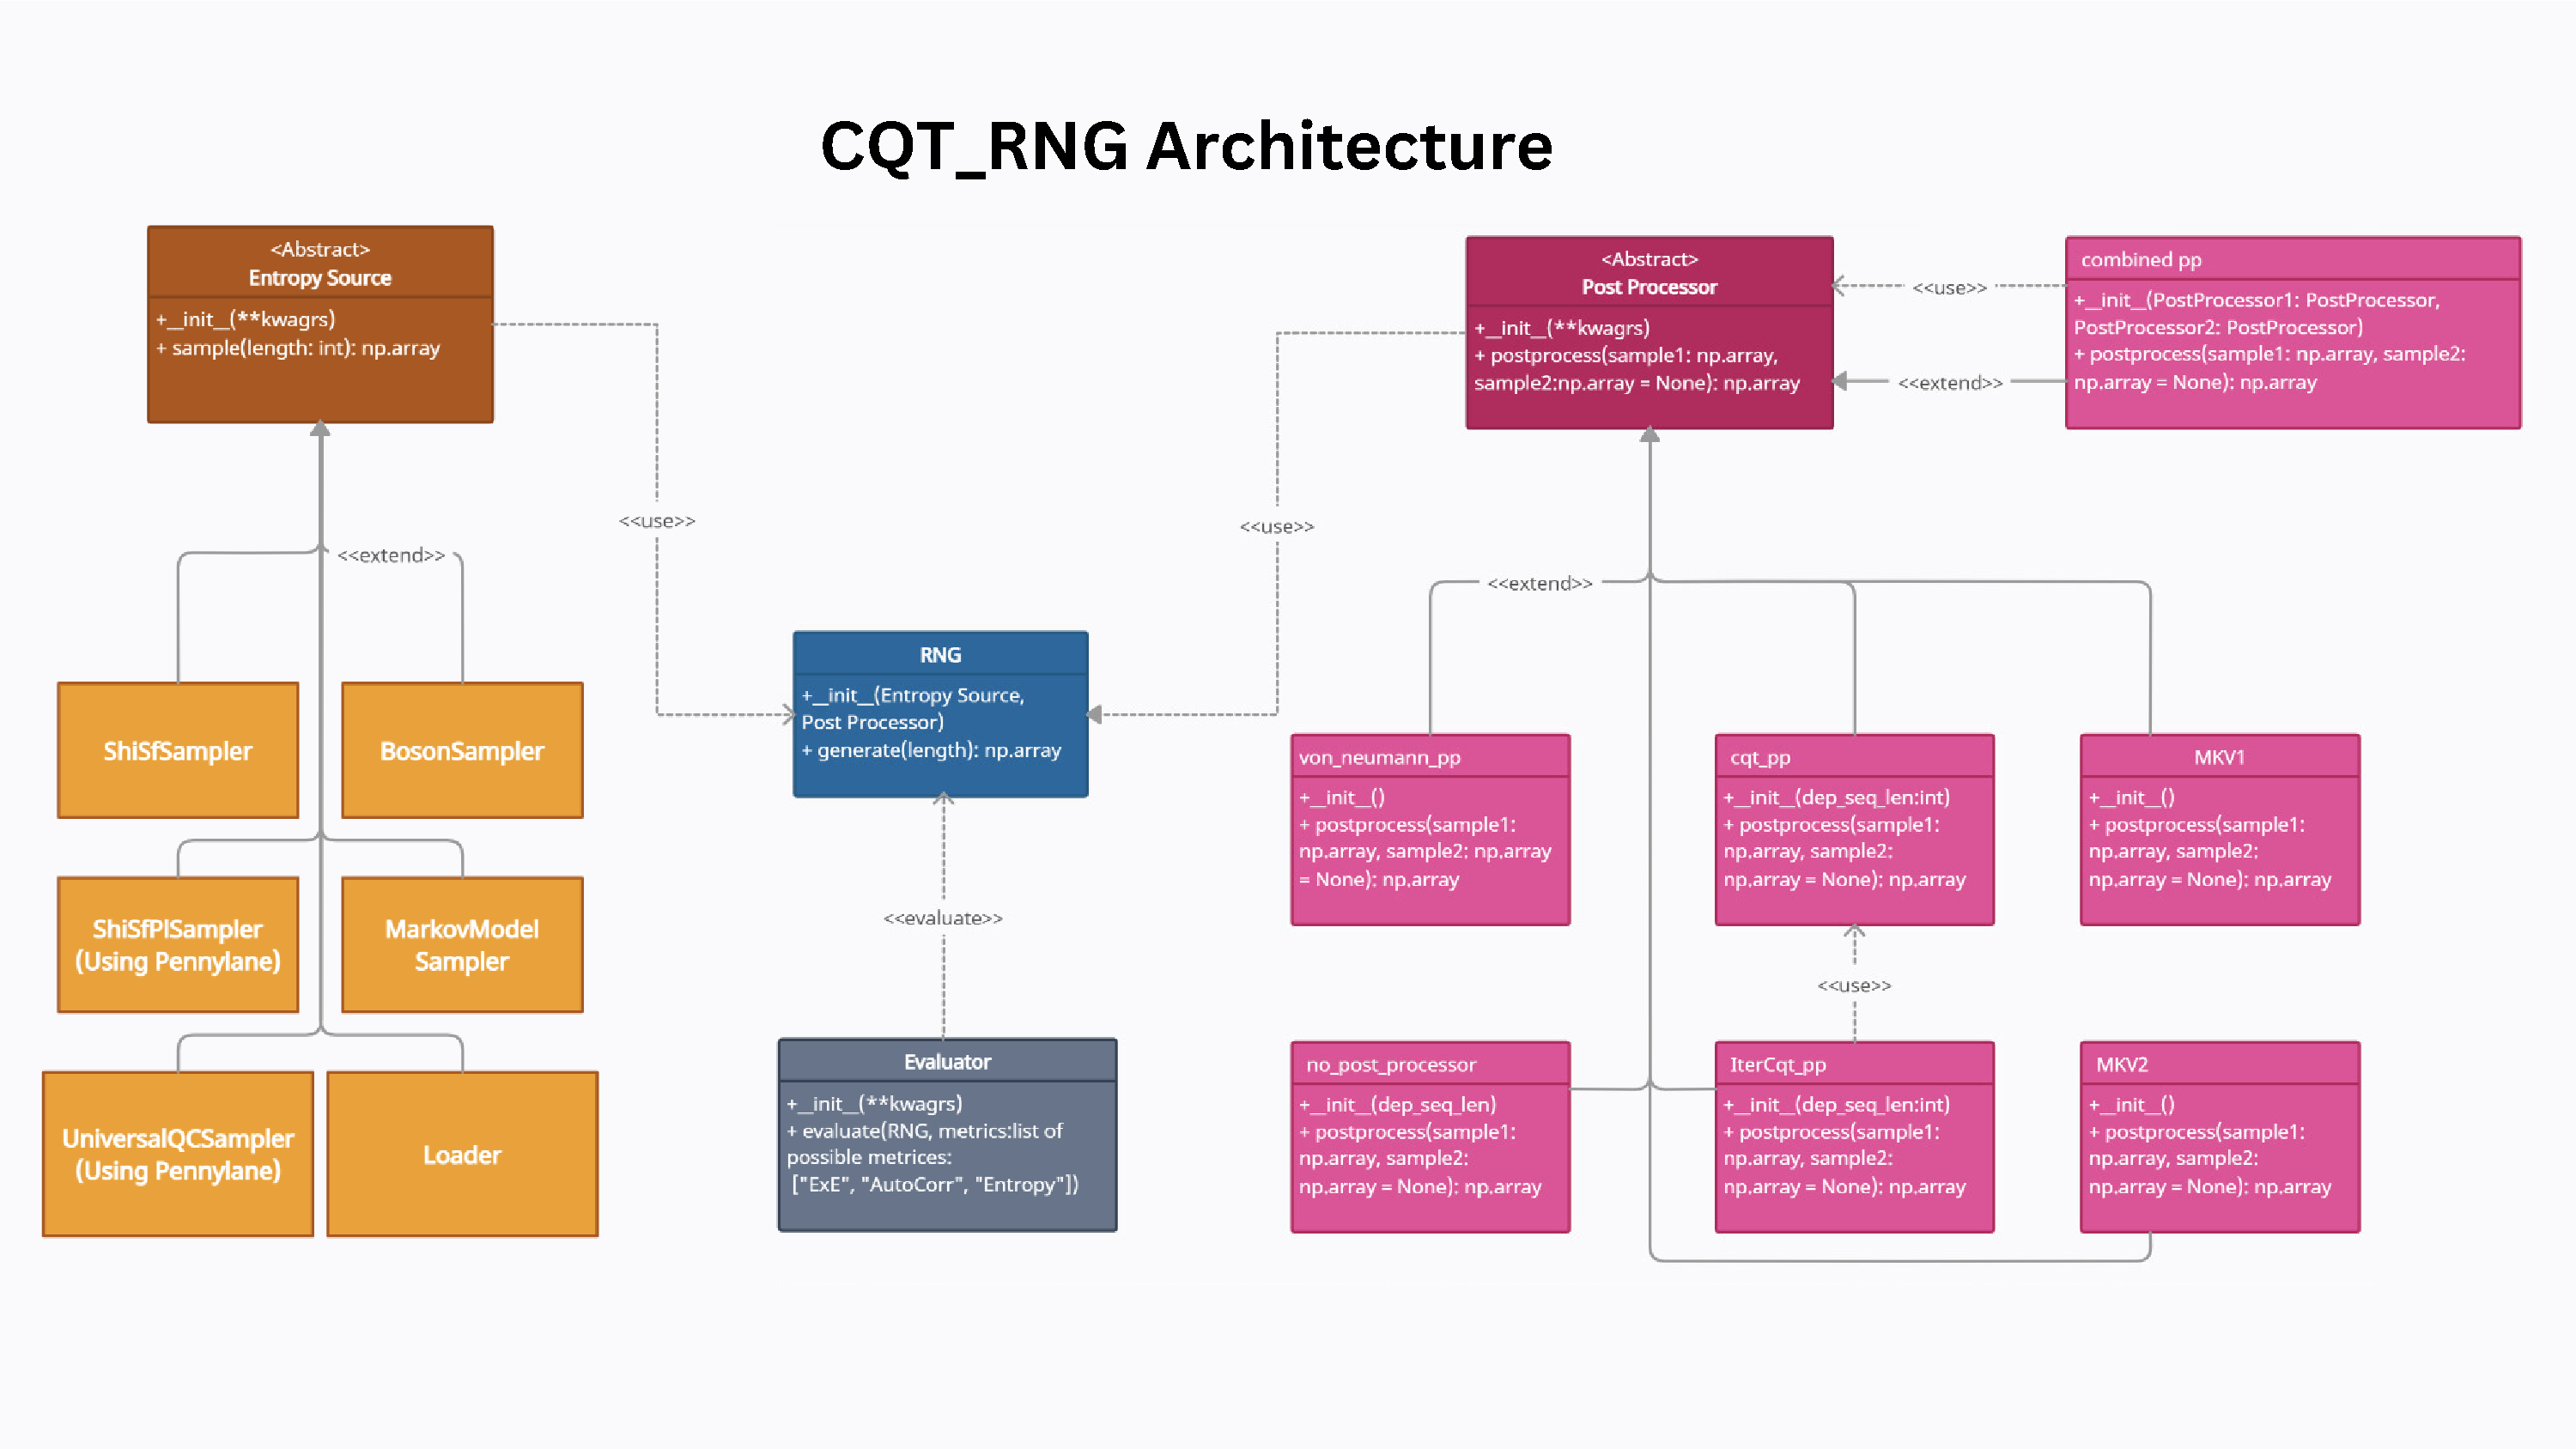
\includegraphics[width = 23cm]{figures/UML.pdf}
    \caption{The cqt\_rng2.0 architecture}
    \label{fig:UML}
\end{figure}
\end{landscape}
\section{This Study's Improvement on the Package: \texttt{cqt\_rng2.0}}

\subsection{Improvements}
\begin{enumerate}
    \item The post-processors can now process a single sample without the need to split it, while the two-sample mode still functions as intended.
    \item Fixed the two-sample length incoherence problem in the Von Neumann post-processor.
    \item Removed outdated modules causing installation errors in \texttt{cqt\_rng}, specifically the two real-device samplers (IBMQ and Borealis) which relied on deprecated packages, and the \texttt{UniversalQCSampler} which used an unsupported version of the IBM API.
    \item Fixed minor bugs and corrected conditional typos.
\end{enumerate}

\subsection{Introduced Novelties}
\begin{enumerate}
    \item Implemented the \texttt{ShiSampler} using Pennylane and a plugin for Strawberry Fields. This implementation was primarily for learning purposes, as writing photonic-based quantum circuits is not yet well-supported in Pennylane.
    \item Re-implemented the \texttt{UniversalQCSampler} using Pennylane, utilizing Hadamard and rotation gates to generate random data.
    \item Introduced the \texttt{Evaluator} module to assess RNG modules based on three functions:
    \begin{itemize}
        \item Extraction Efficiency
        \item Autocorrelation at lag \(k\)
        \item Shannon Entropy of \(n\)-bit words
    \end{itemize}
    \item Introduced the \texttt{MarkovSampler}, enabling the generation of bitlists with defined autocorrelation using the Markov model, which helps in evaluating RNGs.
    \item Added new post-processors such as \texttt{IterCQTPP} and Markov chains with 1-bit and 2-bit histories, as introduced in this study.
    \item Introduced the \texttt{CombinedPostProcessor}, which allows the chaining of two successive post-processors, such as \texttt{MKV+PostProcessor} and others.
    \item Added a new function in the \texttt{CQTPP} package that returns the discarded bits after applying the Von Neumann post-processor, enabling its use in \texttt{IterCQTPP}.
    \item Updated the setup and \texttt{\_\_init\_\_} files to include all required dependencies.
    \item Added the \texttt{generate\_markov\_model\_bitstring} function to the utilities module.
\end{enumerate}
